\mysection{More about pointers}
\myindex{\CLanguageElements!\Pointers}
\label{label_pointers}

\epigraph{The way C handles pointers, for example, was a brilliant innovation;
it solved a lot of problems that we had before in data structuring and
made the programs look good afterwards.}{Donald Knuth, interview (1993)}

For those, who still have hard time understanding \CCpp pointers, here are more examples.
Some of them are weird and serves only demonstration purpose:
use them in production code only if you really know what you're doing.

% subsections:
% TODO proof-reading
\subsubsection{First example}

Strings are objects and are constructed in the same way as other objects (and arrays).


\begin{lstlisting}[style=customjava]
	public static void main(String[] args)
	{
		System.out.println("What is your name?");
		String input = System.console().readLine();
		System.out.println("Hello, "+input);
	}
\end{lstlisting}

\begin{lstlisting}
  public static void main(java.lang.String[]);
    flags: ACC_PUBLIC, ACC_STATIC
    Code:
      stack=3, locals=2, args_size=1
         0: getstatic     #2        // Field java/lang/System.out:Ljava/io/PrintStream;
         3: ldc           #3        // String What is your name?
         5: invokevirtual #4        // Method java/io/PrintStream.println:(Ljava/lang/String;)V
         8: invokestatic  #5        // Method java/lang/System.console:()Ljava/io/Console;
        11: invokevirtual #6        // Method java/io/Console.readLine:()Ljava/lang/String;
        14: astore_1      
        15: getstatic     #2        // Field java/lang/System.out:Ljava/io/PrintStream;
        18: new           #7        // class java/lang/StringBuilder
        21: dup           
        22: invokespecial #8        // Method java/lang/StringBuilder."<init>":()V
        25: ldc           #9        // String Hello, 
        27: invokevirtual #10       // Method java/lang/StringBuilder.append:(Ljava/lang/String;)Ljava/lang/StringBuilder;
        30: aload_1       
        31: invokevirtual #10       // Method java/lang/StringBuilder.append:(Ljava/lang/String;)Ljava/lang/StringBuilder;
        34: invokevirtual #11       // Method java/lang/StringBuilder.toString:()Ljava/lang/String;
        37: invokevirtual #4        // Method java/io/PrintStream.println:(Ljava/lang/String;)V
        40: return        
\end{lstlisting}

The \TT{readLine()} method is called at offset 11, a \emph{reference} to string (which is supplied by the user) 
is then stored at \ac{TOS}.

At offset 14 the \emph{reference} to string is stored in slot 1 of \ac{LVA}.

The string the user entered is reloaded at offset 30 and concatenated with the \q{Hello, } string
using the \TT{StringBuilder} class.

The constructed string is then printed using \TT{println} at offset 37.


\subsection{Another loop optimization}

If you process all elements of some array which happens to be located in global memory, compiler can optimize it.
For example, let's calculate a sum of all elements of array of 128 \emph{int}'s:

\begin{lstlisting}[style=customc]
#include <stdio.h>

int a[128];

int sum_of_a()
{
	int rt=0;
	
	for (int i=0; i<128; i++)
		rt=rt+a[i];

	return rt;
};

int main()
{
	// initialize
	for (int i=0; i<128; i++)
		a[i]=i;
	
	// calculate the sum
	printf ("%d\n", sum_of_a());
};
\end{lstlisting}

Optimizing GCC 5.3.1 (x86) can produce this (\IDA):

\lstinputlisting[style=customasmx86]{advanced/500_loop_optimizations/tmp1.lst}

What the heck is \TT{\_\_libc\_start\_main@@GLIBC\_2\_0} at \TT{0x080484C5}?
This is a label just after end of \TT{a[]} array.
The function can be rewritten like this:

\begin{lstlisting}[style=customc]
int sum_of_a_v2()
{
	int *tmp=a;
	int rt=0;
	
	do
	{
		rt=rt+(*tmp);
		tmp++;
	}
	while (tmp<(a+128));

	return rt;
};
\end{lstlisting}

First version has \emph{i} counter, and the address of each element of array is to be calculated at each iteration.
The second version is more optimized: the pointer to each element of array is always ready and is sliding 4 bytes forward at each iteration.
How to check if the loop is ended?
Just compare the pointer with the address just behind array's end, which is, in our case, is happens to be address of imported \TT{\_\_libc\_start\_main()} function from Glibc 2.0.
Sometimes code like this is confusing, and this is very popular optimizing trick, so that's why I made this example.

My second version is very close to what GCC did, and when I compile it, the code is almost the same as in first version, but two first instructions are swapped:

\lstinputlisting[style=customasmx86]{advanced/500_loop_optimizations/tmp2.lst}

Needless to say, this optimization is possible if the compiler can calculate address of the end of array during compilation time.
This happens if the array is global and it's size is fixed.

However, if the address of array is unknown during compilation, but size is fixed, address of the label just behind array's end can be calculated at the beginning of the loop.
% FIXME <!-- \ref{} to example -->


\subsection{Pointers abuse in Windows kernel}

The resource section of PE executable file in Windows OS is a section containing pictures, icons, strings, etc.
Early Windows versions allowed to address resources only by IDs, but then Microsoft added a way to address them using strings.

So then it would be possible to pass ID or string to 
\href{https://msdn.microsoft.com/en-us/library/windows/desktop/ms648042%28v=vs.85%29.aspx}{FindResource()} function.
Which is declared like this:

\myindex{win32!FindResource()}

\begin{lstlisting}[style=customc]
HRSRC WINAPI FindResource(
  _In_opt_ HMODULE hModule,
  _In_     LPCTSTR lpName,
  _In_     LPCTSTR lpType
);
\end{lstlisting}

\emph{lpName} and \emph{lpType} has \emph{char*} or \emph{wchar*} types, and when someone still wants to pass ID,
he/she have to use
\href{https://msdn.microsoft.com/en-us/library/windows/desktop/ms648029%28v=vs.85%29.aspx}{MAKEINTRESOURCE} macro, like this:

\myindex{win32!MAKEINTRESOURCE()}

\begin{lstlisting}[style=customc]
result = FindResource(..., MAKEINTRESOURCE(1234), ...);
\end{lstlisting}

It's interesting fact that MAKEINTRESOURCE is merely casting integer to pointer.
In MSVC 2013, in the file\\
\emph{Microsoft SDKs\textbackslash{}Windows\textbackslash{}v7.1A\textbackslash{}Include\textbackslash{}Ks.h} we can find this:

\begin{lstlisting}[style=customc]
...

#if (!defined( MAKEINTRESOURCE )) 
#define MAKEINTRESOURCE( res ) ((ULONG_PTR) (USHORT) res)
#endif

...
\end{lstlisting}

Sounds insane. Let's peek into ancient leaked Windows NT4 source code.
In \emph{private/windows/base/client/module.c} we can find \emph{FindResource()} source code:

\begin{lstlisting}[style=customc]
HRSRC
FindResourceA(
    HMODULE hModule,
    LPCSTR lpName,
    LPCSTR lpType
    )

...

{
    NTSTATUS Status;
    ULONG IdPath[ 3 ];
    PVOID p;

    IdPath[ 0 ] = 0;
    IdPath[ 1 ] = 0;
    try {
        if ((IdPath[ 0 ] = BaseDllMapResourceIdA( lpType )) == -1) {
            Status = STATUS_INVALID_PARAMETER;
            }
        else
        if ((IdPath[ 1 ] = BaseDllMapResourceIdA( lpName )) == -1) {
            Status = STATUS_INVALID_PARAMETER;
...
\end{lstlisting}

Let's proceed to \emph{BaseDllMapResourceIdA()} in the same source file:

\begin{lstlisting}[style=customc]
ULONG
BaseDllMapResourceIdA(
    LPCSTR lpId
    )
{
    NTSTATUS Status;
    ULONG Id;
    UNICODE_STRING UnicodeString;
    ANSI_STRING AnsiString;
    PWSTR s;

    try {
        if ((ULONG)lpId & LDR_RESOURCE_ID_NAME_MASK) {
            if (*lpId == '#') {
                Status = RtlCharToInteger( lpId+1, 10, &Id );
                if (!NT_SUCCESS( Status ) || Id & LDR_RESOURCE_ID_NAME_MASK) {
                    if (NT_SUCCESS( Status )) {
                        Status = STATUS_INVALID_PARAMETER;
                        }
                    BaseSetLastNTError( Status );
                    Id = (ULONG)-1;
                    }
                }
            else {
                RtlInitAnsiString( &AnsiString, lpId );
                Status = RtlAnsiStringToUnicodeString( &UnicodeString,
                                                       &AnsiString,
                                                       TRUE
                                                     );
                if (!NT_SUCCESS( Status )){
                    BaseSetLastNTError( Status );
                    Id = (ULONG)-1;
                    }
                else {
                    s = UnicodeString.Buffer;
                    while (*s != UNICODE_NULL) {
                        *s = RtlUpcaseUnicodeChar( *s );
                        s++;
                        }

                    Id = (ULONG)UnicodeString.Buffer;
                    }
                }
            }
        else {
            Id = (ULONG)lpId;
            }
        }
    except (EXCEPTION_EXECUTE_HANDLER) {
        BaseSetLastNTError( GetExceptionCode() );
        Id =  (ULONG)-1;
        }
    return Id;
}
\end{lstlisting}

\emph{lpId} is ANDed with \emph{LDR\_RESOURCE\_ID\_NAME\_MASK}. \\
Which we can find in \emph{public/sdk/inc/ntldr.h}:

\begin{lstlisting}[style=customc]
...

#define LDR_RESOURCE_ID_NAME_MASK 0xFFFF0000

...
\end{lstlisting}

So \emph{lpId} is ANDed with \emph{0xFFFF0000} and if some bits beyond lowest 16 bits are still present,
first half of function is executed (\emph{lpId} is treated as an address of string).
Otherwise---second half (\emph{lpId} is treated as 16-bit value).

Still, this code can be found in Windows 7 kernel32.dll file:

\lstinputlisting[style=customasmx86]{advanced/450_more_ptrs/tmp1.lst}

If value in input pointer is greater than 0x10000, jump to string processing is occurred.
Otherwise, input value of \emph{lpId} is returned as is.
\emph{0xFFFF0000} mask is not used here any more, because this is 64-bit code after all, but still, \emph{0xFFFFFFFFFFFF0000} could work here.

Attentive reader may ask, what if address of input string is lower than 0x10000?
This code relied on the fact that in Windows there are nothing on addresses below 0x10000, at least in Win32 realm.

Raymond Chen \href{https://blogs.msdn.microsoft.com/oldnewthing/20130925-00/?p=3123}{writes} about this:

\begin{framed}
\begin{quotation}
How does MAKE­INT­RESOURCE work? It just stashes the integer in the bottom 16 bits of a pointer, leaving the upper bits zero. This relies on the convention that the first 64KB of address space is never mapped to valid memory, a convention that is enforced starting in Windows 7.
\end{quotation}
\end{framed}

In short words, this is dirty hack and probably one should use it only if there is a real necessity.
Perhaps, \emph{FindResource()} function in past had \emph{SHORT} type for its arguments, and then Microsoft has added a way to pass strings there,
but older code must also be supported.

Now here is my short distilled example:

\begin{lstlisting}[style=customc]
#include <stdio.h>
#include <stdint.h>

void f(char* a)
{
	if (((uint64_t)a)>0x10000)
		printf ("Pointer to string has been passed: %s\n", a);
	else
		printf ("16-bit value has been passed: %d\n", (uint64_t)a);
};

int main()
{
	f("Hello!"); // pass string
	f((char*)1234); // pass 16-bit value
};
\end{lstlisting}

It works!

\subsubsection{Pointers abuse in Linux kernel}

As it has been noted in \href{https://news.ycombinator.com/item?id=11823647}{comments on Hacker News}, Linux kernel also has something like that.

For example, this function can return both error code and pointer:

\begin{lstlisting}[style=customc]
struct kernfs_node *kernfs_create_link(struct kernfs_node *parent,
				       const char *name,
				       struct kernfs_node *target)
{
	struct kernfs_node *kn;
	int error;

	kn = kernfs_new_node(parent, name, S_IFLNK|S_IRWXUGO, KERNFS_LINK);
	if (!kn)
		return ERR_PTR(-ENOMEM);

	if (kernfs_ns_enabled(parent))
		kn->ns = target->ns;
	kn->symlink.target_kn = target;
	kernfs_get(target);	/* ref owned by symlink */

	error = kernfs_add_one(kn);
	if (!error)
		return kn;

	kernfs_put(kn);
	return ERR_PTR(error);
}
\end{lstlisting}

( \url{https://github.com/torvalds/linux/blob/fceef393a538134f03b778c5d2519e670269342f/fs/kernfs/symlink.c#L25} )

\emph{ERR\_PTR} is a macro to cast integer to pointer:

\begin{lstlisting}[style=customc]
static inline void * __must_check ERR_PTR(long error)
{
	return (void *) error;
}
\end{lstlisting}

( \url{https://github.com/torvalds/linux/blob/61d0b5a4b2777dcf5daef245e212b3c1fa8091ca/tools/virtio/linux/err.h} )

This header file also has a macro helper to distinguish error code from pointer:

\begin{lstlisting}[style=customc]
#define IS_ERR_VALUE(x) unlikely((x) >= (unsigned long)-MAX_ERRNO)
\end{lstlisting}

This means, error codes are the ``pointers'' which are very close to -1 and, hopefully, there are nothing in kernel memory
on the addresses like 0xFFFFFFFFFFFFFFFF, 0xFFFFFFFFFFFFFFFE, 0xFFFFFFFFFFFFFFFD, etc.

Much more popular solution is to return \emph{NULL} in case of error and to pass error code via additional argument.
Linux kernel authors don't do that, but everyone who use these functions must always keep in mind that returning pointer
must always be checked with \emph{IS\_ERR\_VALUE} before dereferencing.

For example:

\begin{lstlisting}[style=customc]
	fman->cam_offset = fman_muram_alloc(fman->muram, fman->cam_size);
	if (IS_ERR_VALUE(fman->cam_offset)) {
		dev_err(fman->dev, "%s: MURAM alloc for DMA CAM failed\n",
			__func__);
		return -ENOMEM;
	}
\end{lstlisting}

( \url{https://github.com/torvalds/linux/blob/aa00edc1287a693eadc7bc67a3d73555d969b35d/drivers/net/ethernet/freescale/fman/fman.c#L826} )

\subsubsection{Pointers abuse in UNIX userland}

\myindex{UNIX!mmap()}
mmap() function returns -1 in case of error (or \TT{MAP\_FAILED}, which equals to -1).
Some people say, mmap() can map a memory at zeroth address in rare situations, so it can't use 0 or NULL as error code.


\subsection{Null pointers}

\subsubsection{``Null pointer assignment'' error of MS-DOS era}

\myindex{MS-DOS}
Oldschool readers may recall a weird error message of MS-DOS era: ``Null pointer assignment''.
What does it mean?

It's not possible to write a memory at zero address in *NIX and Windows OSes, but it was possible to do so in MS-DOS due to absence of memory protection whatsoever.

\myindex{Turbo C++}
\myindex{Borland C++}
So I've pulled my ancient Turbo C++ 3.0 (later it was renamed to Borland C++) from early 1990s and tried to compile this:

\begin{lstlisting}[style=customc]
#include <stdio.h>

int main()
{
	int *ptr=NULL;
	*ptr=1234;
	printf ("Now let's read at NULL\n");
	printf ("%d\n", *ptr);
};
\end{lstlisting}

Hard to believe, but it works, with error upon exit, though:

\begin{lstlisting}[caption=Ancient Turbo C 3.0]
C:\TC30\BIN\1
Now let's read at NULL
1234
Null pointer assignment

C:\TC30\BIN>_
\end{lstlisting}

Let's dig deeper into the source code of \ac{CRT} of Borland C++ 3.1, file \emph{c0.asm}:

\lstinputlisting[style=customasmx86]{advanced/450_more_ptrs/tmp2.lst}

The MS-DOS memory model was really weird (\myref{8086_memory_model}) and probably not worth looking into it unless you're fan of retrocomputing or retrogaming.
One thing we have to keep in mind is that memory segment (included data segment) in MS-DOS is a memory segment in which code or data is stored,
but unlike ``serious'' \ac{OS}es, it's started at address 0.

And in Borland C++ \ac{CRT}, the data segment is started with 4 zero bytes and the copyright string ``Borland C++ - Copyright 1991 Borland Intl.''.
The integrity of the 4 zero bytes and text string is checked upon exit, and if it's corrupted, the error message is displayed.

But why? Writing at null pointer is common mistake in \CCpp, and if you do so in *NIX or Windows, your application will crash.
MS-DOS has no memory protection, so \ac{CRT} has to check this post-factum and warn about it upon exit.
If you see this message, this means, your program at some point has written at address 0.

Our program did so. And this is why 1234 number has been read correctly: because it was written at the place of the first 4 zero bytes.
Checksum is incorrect upon exit (because the number has been left there), so error message has been displayed.

Am I right?
I've rewritten the program to check my assumptions:

\begin{lstlisting}[style=customc]
#include <stdio.h>

int main()
{
	int *ptr=NULL;
	*ptr=1234;
	printf ("Now let's read at NULL\n");
	printf ("%d\n", *ptr);
	*ptr=0; // psst, cover our tracks!
};
\end{lstlisting}

This program executes without error message upon exit.

Though method to warn about null pointer assignment is relevant for MS-DOS,
perhaps, it can still be used today in low-cost \ac{MCU}s with no memory protection and/or \ac{MMU}.

\subsubsection{Why would anyone write at address 0?}

But why would sane programmer write a code which writes something at address 0?
It can be done accidentally: for example, a pointer must be initialized to newly allocated memory block and then passed to some function which returns data through pointer.

\begin{lstlisting}[style=customc]
int *ptr=NULL;

... we forgot to allocate memory and initialize ptr

strcpy (ptr, buf); // strcpy() terminates silently because MS-DOS has no memory protection
\end{lstlisting}

Even worse:

\begin{lstlisting}[style=customc]
int *ptr=malloc(1000);

... we forgot to check if memory has been really allocated: this is MS-DOS after all and computers had small amount of RAM,
... and RAM shortage was very common.
... if malloc() returned NULL, the ptr will also be NULL.

strcpy (ptr, buf); // strcpy() terminates silently because MS-DOS has no memory protection
\end{lstlisting}

\subsubsection{Writing on 0th address on purpose}
\label{dmalloc_KILL_PROCESS}

\myindex{dmalloc}
\myindex{Core dump}
Here is an example from dmalloc\footnote{\url{http://dmalloc.com/}},
a portable way of generating core dump, if other ways are not available:

\lstinputlisting{advanced/450_more_ptrs/dmalloc_KILL_PROCESS}

\subsubsection{NULL in \CCpp}

NULL in C/C++ is just a macro which is often defined like this:

\begin{lstlisting}[style=customc]
#define NULL  ((void*)0)
\end{lstlisting}
( \href{https://github.com/wzhy90/linaro_toolchains/blob/8ff8ae680bac04558d10cc9626e12c4c2f6c1348/arm-cortex_a15-linux-gnueabihf/libc/usr/include/libio.h#L70}{libio.h file} )

\emph{void*} is a data type reflecting the fact it's the pointer, but to a value of unknown data type (\emph{void}).

NULL is usually used to show absence of an object.
For example, you have a single-linked list, and each node has a value (or pointer to a value) and \emph{next} pointer.
To show that there are no next node, 0 is stored to \emph{next} field.
(Other solutions are just worse.)
Perhaps, you may have some crazy environment where you need to allocate memory blocks at zero address. How would you indicate absence of the next node?
Some kind of \emph{magic number}? Maybe -1? Or maybe using additional bit?

In Wikipedia we may find this:

\begin{framed}
\begin{quotation}
In fact, quite contrary to the zero page's original preferential use, some modern operating systems such as FreeBSD, Linux and Microsoft Windows[2] actually make the zero page inaccessible to trap uses of NULL pointers. 
\end{quotation}
\end{framed}
( \url{https://en.wikipedia.org/wiki/Zero_page} )

\subsubsection{Null pointer to function}

It's possible to call function by its address.
For example, I compile this by MSVC 2010 and run it in Windows 7:

\begin{lstlisting}[style=customc]
#include <windows.h>
#include <stdio.h>

int main()
{
	printf ("0x%x\n", &MessageBoxA);
};
\end{lstlisting}

The result is \emph{0x7578feae} and doesn't changing after several times I run it,
because user32.dll (where MessageBoxA function resides) is always loads at the same address.
And also because \ac{ASLR} is not enabled (result would be different each time in that case).

Let's call \emph{MessageBoxA()} by address:

\begin{lstlisting}[style=customc]
#include <windows.h>
#include <stdio.h>

typedef int (*msgboxtype)(HWND hWnd, LPCTSTR lpText, LPCTSTR lpCaption,  UINT uType);

int main()
{
	msgboxtype msgboxaddr=0x7578feae;

	// force to load DLL into process memory, 
	// since our code doesn't use any function from user32.dll, 
	// and DLL is not imported
	LoadLibrary ("user32.dll");

	msgboxaddr(NULL, "Hello, world!", "hello", MB_OK);
};
\end{lstlisting}

Weird, but works in Windows 7 x86.

This is commonly used in shellcodes, because it's hard to call DLL functions by name from there.
And \ac{ASLR} is a countermeasure.

Now what is really weird, some embedded C programmers may be familiar with a code like that:

\begin{lstlisting}[style=customc]
int reset()
{
	void (*foo)(void) = 0;
	foo();
};
\end{lstlisting}

Who will want to call a function at address 0?
This is portable way to jump at zero address.
Many low-cost cheap microcontrollers also have no memory protection or \ac{MMU} and after reset, they start to execute code at address 0, where some kind of initialization code is stored.
So jumping to address 0 is a way to reset itself.
One could use inline assembly, but if it's not possible, this portable method can be used.

It even compiles correctly by my GCC 4.8.4 on Linux x64:

\begin{lstlisting}[style=customasmx86]
reset:
        sub     rsp, 8
        xor     eax, eax
        call    rax
        add     rsp, 8
        ret
\end{lstlisting}

The fact that stack pointer is shifted is not a problem: initialization code in microcontrollers usually completely ignores registers and \ac{RAM} state and boots from scratch.

And of course, this code will crash on *NIX or Windows because of memory protection and even in absence of protection, there are no code at address 0.

GCC even has non-standard extension, allowing to jump to a specific address rather than call a function there:
\url{http://gcc.gnu.org/onlinedocs/gcc/Labels-as-Values.html}.


\subsection{Array as function argument}

Someone may ask, what is the difference between declaring function argument type as array and as pointer?

As it seems, there are no difference at all:

\begin{lstlisting}[style=customc]
void write_something1(int a[16])
{
	a[5]=0;
};

void write_something2(int *a)
{
	a[5]=0;
};

int f()
{
	int a[16];
	write_something1(a);
	write_something2(a);
};
\end{lstlisting}

Optimizing GCC 4.8.4:

\begin{lstlisting}[style=customasmx86]
write_something1:
        mov     DWORD PTR [rdi+20], 0
        ret

write_something2:
        mov     DWORD PTR [rdi+20], 0
        ret
\end{lstlisting}

But you may still declare array instead of pointer for self-documenting purposes, if the size of array is always fixed.
And maybe, some static analysis tool will be able to warn you about possible buffer overflow.
Or is it possible with some tools today?

Some people, including Linus Torvalds, criticizes this \CCpp feature: \url{https://lkml.org/lkml/2015/9/3/428}.

C99 standard also have \emph{static} keyword \InSqBrackets{\CNineNineStd{} 6.7.5.3}:

\begin{framed}
\begin{quotation}
If the keyword static also appears  within the [ and ] of the array type derivation, then for each call to the function, the value of the corresponding actual argument shall provide access to the first element of an array with at least as many elements as specified by the size expression.
\end{quotation}
\end{framed}


\subsection{Pointer to a function}

A function name in \CCpp without brackets, like ``printf'' is a pointer to function of \emph{void (*)()} type.
Let's try to read function's contents and patch it:

\lstinputlisting[style=customc]{advanced/450_more_ptrs/6.c}

It tells, that the first 3 bytes of functions are \TT{55 89 e5}.
Indeed, these are opcodes of \INS{PUSH EBP} and \INS{MOV EBP, ESP} instructions (these are x86 opcodes).
But then our program crashes, because \emph{text} section is readonly.

We can recompile our example and make \emph{text} section writable
\footnote{\url{http://stackoverflow.com/questions/27581279/make-text-segment-writable-elf}}:

\begin{lstlisting}
gcc --static -g -Wl,--omagic -o example example.c
\end{lstlisting}

That works!

\begin{lstlisting}
we are in print_something()
first 3 bytes: 55 89 e5...
going to call patched print_something():
it must exit at this point
\end{lstlisting}


\subsection{Pointer to a function: copy protection}
\myindex{\SoftwareCracking}

A software cracker can find a function that checks protection and return \emph{true} or \emph{false}.
He/she then can put \TT{XOR EAX,EAX / RETN} or \TT{MOV EAX, 1 / RETN} there.

Can you check integrity of the function?
As it turns out, this can be done easily.

According to objdump, the first 3 bytes of \verb|check_protection()| are 0x55 0x89 0xE5 (given the fact this is non-optimizing GCC):

\lstinputlisting[style=customc]{advanced/450_more_ptrs/61.c}

\lstinputlisting[style=customc]{advanced/450_more_ptrs/61_objdump.txt}

If someone would patch the beginning of the \verb|check_protection()| function,
your program can do something mean, maybe exit suddenly.
To find such a trick, a cracker can set a memory read breakpoint on the address of the function's beginning.
(\tracer has BPMx options for that.)


\subsection{Pointer to a function: a common bug (or typo)}

A notorious bug/typo:

\lstinputlisting[style=customc]{advanced/450_more_ptrs/62.c}

Since the function's name alone is interpreted as a pointer to function, or its address,\\
the \verb|if(function_name)| statement is like \verb|if(true)|.

Unfortunately, a \CCpp compiler wouldn't issue a warning.


\subsection{Pointer as object identificator}

Both assembly language and C has no \ac{OOP} features, but it's possible to write a code in \ac{OOP} style
(just treat structure as an object).

It's interesting, that sometimes, pointer to an object (or its address) is called as ID
(in sense of data hiding/encapsulation).

\myindex{win32!LoadLibrary()}
\myindex{win32!GetProcAddress()}
For example, LoadLibrary(), according to \ac{MSDN}, returns ``handle to the module''
\footnote{\url{https://msdn.microsoft.com/ru-ru/library/windows/desktop/ms684175(v=vs.85).aspx}}.
Then you pass this ``handle'' to other functions like GetProcAddress().
But in fact, LoadLibrary() returns pointer to DLL file mapped into memory
\footnote{\url{https://blogs.msdn.microsoft.com/oldnewthing/20041025-00/?p=37483}}.
You can read two bytes from the address LoadLibrary() returns, and that would be ``MZ'' (first two bytes of any
.EXE/.DLL file in Windows).

\myindex{win32!HMODULE}
\myindex{win32!HINSTANCE}
Apparently, Microsoft ``hides'' that fact to provide better forward compatibility.
Also, HMODULE and HINSTANCE data types had another meaning in 16-bit Windows.

Probably, this is reason why \printf has ``\%p'' modifier, which is used for printing pointers (32-bit integers
on 32-bit architectures, 64-bit on 64-bit, etc) in hexadecimal form.
Address of a structure dumped into debug log may help in finding it in another place of log.

\myindex{SQLite}
Here is also from SQLite source code:

\begin{lstlisting}

...

struct Pager {
  sqlite3_vfs *pVfs;          /* OS functions to use for IO */
  u8 exclusiveMode;           /* Boolean. True if locking_mode==EXCLUSIVE */
  u8 journalMode;             /* One of the PAGER_JOURNALMODE_* values */
  u8 useJournal;              /* Use a rollback journal on this file */
  u8 noSync;                  /* Do not sync the journal if true */

....

static int pagerLockDb(Pager *pPager, int eLock){
  int rc = SQLITE_OK;

  assert( eLock==SHARED_LOCK || eLock==RESERVED_LOCK || eLock==EXCLUSIVE_LOCK );
  if( pPager->eLock<eLock || pPager->eLock==UNKNOWN_LOCK ){
    rc = sqlite3OsLock(pPager->fd, eLock);
    if( rc==SQLITE_OK && (pPager->eLock!=UNKNOWN_LOCK||eLock==EXCLUSIVE_LOCK) ){
      pPager->eLock = (u8)eLock;
      IOTRACE(("LOCK %p %d\n", pPager, eLock))
    }
  }
  return rc;
}

...

  PAGER_INCR(sqlite3_pager_readdb_count);
  PAGER_INCR(pPager->nRead);
  IOTRACE(("PGIN %p %d\n", pPager, pgno));
  PAGERTRACE(("FETCH %d page %d hash(%08x)\n",
               PAGERID(pPager), pgno, pager_pagehash(pPg)));

...

\end{lstlisting}


\subsection{Oracle RDBMS and a simple garbage collector for C/C++}

There was a time, when the author of these lines tried to learn more about Oracle RDBMS, searching for vulnerabilities, etc.
This is a huge piece of software, and a typical function can take very large nested objects as arguments.
And I wanted to dump these objects, as trees (or graphs).

Also, I tracked all memory allocations/deallocations by intercepting memory allocating/deallocating functions.
And when a function to be intercepted getting a pointer to a block in memory, I search for the block in a list of blocks allocated.
I'm getting its size + short name of block
(this is like "tagging" in Windows OS kernel\footnote{Read more about comments in allocated blocks: \CNotes{} \url{http://yurichev.com/C-book.html}}).

Given a block, I can scan it for 32-bit words (on 32-bit OS) or for 64-bit words (on 64-bit OS).
Each word can be a pointer to another block.
And if it is so (I find this another block in my records), I can process it recursively.

\myindex{GraphViz}
And then, using GraphViz, I could render such a diagrams:

\begin{figure}[H]
\centering
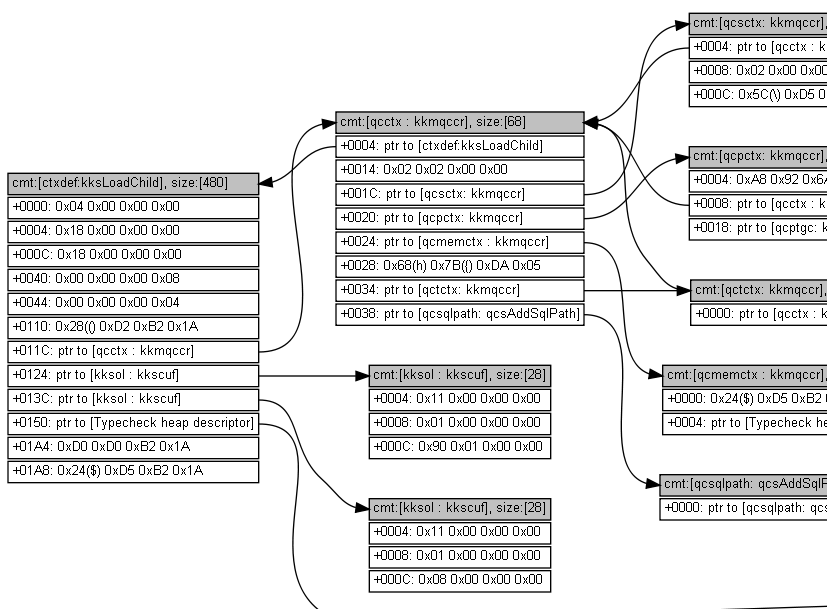
\includegraphics[width=\textwidth]{advanced/450_more_ptrs/oracle2_crop.png}
\end{figure}

Bigger pictures:
\href{\RepoURL/advanced/450_more_ptrs/oracle1.png}{1},
\href{\RepoURL/advanced/450_more_ptrs/oracle2.png}{2}.

This is quite impressive, given the fact that I had no information about data types of all these structures.
But I could get some information from it.

\subsubsection{Now the garbage collector for C/C++: Boehm GC}

\myindex{Garbage collector}
If you use a block allocated in memory, its address has to be present somewhere, as a pointer in some structure/array in another allocated block,
or in globally allocated structure, or in local variable in stack.
If there are no pointer to a block, you can call it "orphan", and it will be a reason of memory leak.

And this is what \ac{GC} does.
It scans all blocks (because it keep tabs on all blocks allocated) for pointers.
It's important to understand, that it has no idea of data types of all these structure fields in blocks---this is important, \ac{GC} has no information about types.
It just scans blocks for 32-bit of 64-bit words and see, if they could be a pointers to another block(s).
It also scans stack.
It treats allocated blocks and stack as arrays of words, some of which may be pointers.
And if it found a block allocated, which is "orphaned", i.e., there are no pointer(s) to it from another block(s) or stack, this block considered unneeded, to be freed.
Scanning process takes time, and this is what for \ac{GC}s are criticized.

\myindex{Boehm garbage collector}
Also, \ac{GC} like Boehm GC\footnote{\url{https://www.hboehm.info/gc/}} (for pure C) has function like \verb|GC_malloc_atomic()|---using it, you declare that the block allocated
using this function will never contain any pointer(s) to other block(s).
Maybe this could be a text string, or other type of data.
(Indeed, \verb|GC_strdup()| calls \verb|GC_malloc_atomic()|.)
\ac{GC} will not scan it.

% Even more: if \ac{GC}'s memory allocator thinks it can find a better place for a block, it can \emph{move} it to another place, and then fix (rewrite) all addresses,
% pointing to it, in all other blocks and in stack.



